\documentclass{beamer}
\usepackage{listings}
\lstset{
%language=C,
frame=single, 
breaklines=true,
columns=fullflexible
}
\usetheme[progressbar=frametitle]{metropolis}
\usepackage{appendixnumberbeamer}

\usepackage{booktabs}
\usepackage[scale=2]{ccicons}
\newenvironment{subcolumns}[1]
 {\valign\bgroup\hsize=#1##\cr}
 {\crcr\egroup}
\newcommand{\nextsubcolumn} {\cr\noalign{\hfill}}
\newcommand{\nextsubfigure}{\vfill}
\usepackage{pgfplots}
\usepgfplotslibrary{dateplot}

\usepackage{xspace}
\newcommand{\themename}{\textbf{\textsc{metropolis}}\xspace}
\usepackage{subcaption}
\usepackage{url}

\usepackage{tikz}
\usetikzlibrary{arrows.meta,positioning}
\usepackage{pgfplots}
\pgfplotsset{compat=1.17}
\usepackage{tkz-fct}
\usepackage{mathrsfs}
\usepackage{txfonts}
\usepackage{tkz-euclide} 
\usetikzlibrary{calc,math}
\usepackage{float}
\newcommand\norm[1]{\left\lVert#1\right\rVert}
\renewcommand{\vec}[1]{\mathbf{#1}}
\providecommand{\pr}[1]{\ensuremath{\Pr\left(#1\right)}}
\usepackage[export]{adjustbox}
\usepackage[utf8]{inputenc}
\usepackage{amsmath}
\usepackage{mathtools}
\usepackage{xfrac}
\newcommand{\SubItem}[1]{
    {\setlength\itemindent{15pt} \item[-] #1}
}
\title{Using Regularized SVD for Recommender Systems (iterative method)}
\subtitle{MA5120 - Numeric Linear Algebra}
\date{\today}

\author{Prajwaldeep and Vishwanath}
%\institute{Indian Institute of Technology Hyderabad}
\titlegraphic{\hfill
\includegraphics[height=1.5cm]{iith logo.png}}

\begin{document}
\metroset{block=fill}
\begin{frame}
\titlepage
\end{frame}
\begin{frame}{Team Members}
\begin{itemize}
    \item Mulugu Vishwanath Sharma - MA20BTECH11010
    \item Prajwaldeep Kamble - MA20BTECH11013
\end{itemize}
\end{frame}
\begin{frame}
\section{Introduction}
\end{frame}
\begin{frame}{Introduction}
   \begin{block}{Abstract}
    This presentaion is part of course project for MA5120 - Numeric Linear Algebra. The project is based on the paper "Using Regularized SVD and Application to Recommender Systems" by Shuai Zheng, Chris Ding and Feiping Nie. 
    The paper is about the use of Regularized SVD for Recommender Systems and How we could optimize the RSVD by using the Iterative method. We implemented the alogorith in Python and checked it on actual movie Dataset. 
   \end{block} 
\end{frame}
\begin{frame}{Introduction}
   \begin{block}{About Recommender Systems}
    The Recommender Systems are a really important application Numeric Linear Algebra in the modern world.
    they're used extensively by the Streaming platforms (like Netflix and YouTube), movie rating websites (like imdb and my anime list) as well as E-commerce platforms like amazon/flipkart. 
    In our class this was mentioned as an application of the SVD and referred to as 'The Netflix Problem'. Netfix also awards the 'Netflix Prize' for best collaborative flitering alogorithm.
   \end{block} 
\end{frame}
\begin{frame}{Introduction}
    \begin{block}{collaborative Flitering Alogorithms}
    The collaborative flitering alogorithms are used to make predictions about the user's interests by collecting information from many users (collaborating). The information collected is used to predict the items (movies, songs, products, etc) that the user might like.
    Unlike the content-based recommender systems, the collaborative flitering alogorithms do not require the item's metadata.
    It uses the data from other users who liked the same item to predict the user's interest.
    \end{block} 
 \end{frame}
 \begin{frame}{Introduction}
    \begin{block}{Regularized SVD}
    The Regularized SVD is a method to approximate a matrix by using the SVD of the matrix. It is used to reduce the dimensionality of the data. It is also used to remove noise from the data.
    The main idea behind the RSVD is to add a regularization term to the SVD. The regularization term is used to penalize the large values in the matrix.
    The RSVD is used in many applications like Recommender Systems, Image Processing, etc.
    It's primary advantage over the SVD is that it is more robust to noise and overfitting.
    \end{block} 
 \end{frame}

 \begin{frame}{Introduction}
    \begin{block}{Regularized SVD}
    Assume there is a matrix $X \in \mathbb{R}^{m \times n}$. Regularized SVD (RSVD) tries to find low-rank approximation using regularized factor matrices $U$ and $V$. The objective function is proposed as
    \begin{equation}
        J_1 = \norm{X - UV^T}_F^2 + \lambda\norm{U}_F^2 + \lambda\norm{V}_F^2 \label{eq:1}
    \end{equation}
    where low-rank regularized factor matrices $U \in \mathbb{R}^{n \times k}$ and $V \in \mathbb{R}^{m \times k}$, $k$ is the Number of latent features of the moves that we are considering. Minimizing eq:$\ref{eq:1}$ is a multi-variable problem.
    \end{block}
 \end{frame}

\begin{frame}
\section{Data Collection}
\end{frame}
\begin{frame}{Data Collection}
   \textbf{The Dataset-1}
     \begin{itemize}
    \item The dataset is 'The movies dataset' from Kaggle. It contains the data of 3,000 movies released on or before July 2017 along with ratings of 1081 users.
    \item The dataset contains the following information about the movies: Ratings, Budget, Revenue, Genres, Cast, Crew, etc.; metadata about the movies, Userid, Credits etc..
    \item But We'll be using only the Userid and Ratings from the dataset. As we're using the collaborative flitering alogorithm. We don't need the metadata of the movies.
\end{itemize}
\end{frame}

\begin{frame}{Data Collection}
    \textbf{The Dataset-2}
      \begin{itemize}
     \item The dataset is "TMBD 5000 Dataset" The dataset is very Similar to the previous dataset
     \item It contains all attributes like metadata, cast, crew, budget, revenue, release dates, languages, production companies, countries, TMDB vote counts and vote averages.
     \item But for collaborative flitering alogorithm we'll be using only the Userid and Ratings from the dataset. We don't need the metadata of the movies.
     \item It's Glimpse is Similar to the previous dataset.
 \end{itemize}
 \end{frame}

\begin{frame}{Movie Dataset-1}
\begin{figure}[htp]
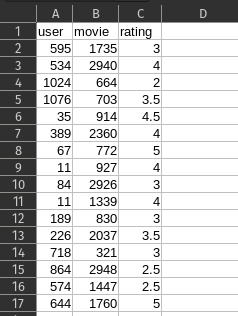
\includegraphics[width=1.05\textwidth]{dataset.png}
\caption{UsersId, movieId and Ratings}
\end{figure}  
\end{frame}



\begin{frame}{Defining variables}
The below representations of all the variables are used in the presentation.
\begin{itemize}
    \item $m$ - Number of users
    \item $n$ - Number of movies
    \item $k$ - Number of latent features
    \item $X$ - $m \times n$ matrix of ratings, where $X_{ij}$ is the rating given by user $i$ to movie $j$
    \item $U$ - $m \times k$ matrix of user features, where $U_{ik}$ is the strength of association of user $i$ with latent feature $k$
    \item $V$ - $n \times k$ matrix of movie features, where $V_{jk}$ is the strength of association of movie $j$ with latent feature $k$
\end{itemize}
\end{frame}

\begin{frame}
\section{Alogorithms}
\end{frame}

\begin{frame}
\section{Iterative way of finding U and V}
\end{frame}

\begin{frame}{Iterative way of finding U and V}
    \begin{itemize}
        \item The objective function is proposed as $J_1 = \norm{X - UV^T}_F^2 + \lambda\norm{U}_F^2 + \lambda\norm{V}_F^2$
        \item On taking the partial derivative of the above equation with respect to U and equating it to zero, we get $$U = (XV)(VV^T + \lambda I)^{-1}$$
        \item On taking the partial derivative of the above equation with respect to V and equating it to zero, we get $$V = (X^TU)(UU^T + \lambda I)^{-1}$$
    \end{itemize}


\end{frame}

\begin{frame}{Iterative way of finding U and V}
    \textbf{Step 1:} Initialize $V$ with random values.\\
    \textbf{Step 2:} Calculate $U$ using the equation $U = (XV)(VV^T + \lambda I)^{-1}$\\
    \textbf{Step 3:} Calculate $V$ using the equation $V = (X^TU)(UU^T + \lambda I)^{-1}$\\
    \textbf{Step 4:} Repeat Step 2 and Step 3 until convergence.\\
\end{frame}

\begin{frame}{RSVD in Subspace of SVD}
    Let $F \Sigma G^{T}$ is the SVD of the matrix $X$. And the optimal values of RSVD be $U^*$ and $V^*$. Then the following holds true:\\
    \begin{align}
            U^* &= F_K * \Omega\\
            V^* &= G_K * \Omega\\
    \end{align}
    where,
    \begin{align}
        F_K &= F[:, 1:K]\\
        G_K &= G[:, 1:K]\\
        \Omega &= \sqrt{\Sigma - \lambda I_K}
    \end{align}
\end{frame}

\begin{frame}{Computational Complexity}
    \begin{itemize}
        \item The computational complexity of the RSVD is O(k(m+n)\emph{min}(m, n)).
        \item But the iterative way of finding U and V is computationally less expensive than the RSVD because the term $VV^T + \lambda I$ is much faster to converge than SVD.
    \end{itemize}
\end{frame}

\begin{frame}{Results}
    \begin{figure}[htp]
    \includegraphics[width=0.9\textwidth]{/home/pluton/Documents/Desktop Files/sem-6/NLA/Movie_recommendations/Images-Data/K=3.png}
    \caption{Convergence of RSVD on dataset-1 for k=3}
    \end{figure}
\end{frame}

\begin{frame}{Results}
    \begin{figure}[htp]
    \includegraphics[width=0.9\textwidth]{/home/pluton/Documents/Desktop Files/sem-6/NLA/Movie_recommendations/Images-Data/K=10.png}
    \caption{Convergence of RSVD on dataset-1 for k=10}
    \end{figure}
\end{frame}

\begin{frame}{Results}
    \begin{figure}[htp]
    \includegraphics[width=0.9\textwidth]{/home/pluton/Documents/Desktop Files/sem-6/NLA/Movie_recommendations/Images-tmdb/K=3.png}
    \caption{Convergence of RSVD on dataset-2 for k=3}
    \end{figure}
\end{frame}

\begin{frame}{Results}
    \begin{figure}[htp]
    \includegraphics[width=0.9\textwidth]{/home/pluton/Documents/Desktop Files/sem-6/NLA/Movie_recommendations/Images-tmdb/K=10.png}
    \caption{Convergence of RSVD on dataset-2 for k=10}
    \end{figure}
\end{frame}
\end{document}